\documentclass[11pt,letterpaper]{article}
\usepackage{fullpage}
\usepackage[top=2cm, bottom=4.5cm, left=2.5cm, right=2.5cm]{geometry}
\usepackage{amsmath,amsfonts,amssymb}
\usepackage{lastpage}
\usepackage[inline]{enumitem}
\usepackage{fancyhdr}
\usepackage{mathrsfs}
\usepackage{xcolor}
\usepackage{graphicx}
\usepackage{hyperref}
\usepackage{subcaption}
\hypersetup{colorlinks=true, linkcolor=blue, linkbordercolor={0 0 1}}

\renewcommand{\arraystretch}{1.75}

\setlength{\parindent}{0.0in}
\setlength{\parskip}{0.05in}

\newcommand{\its}{\item[\tiny\textbullet]}

\pagestyle{fancyplain}
\lhead{Brad Cownden}
\chead{}
\rhead{July 2, 2020}
\cfoot{\small\thepage}
\headsep 36pt

\begin{document}
\vspace{.2in}
\begin{center}
    {\bf GPU Solutions for PSCAD: IT17112}
\end{center}

\vspace{.25in}

\begin{tabular}{| p{0.2\textwidth} | p{0.75\textwidth} |}
	\hline
	Reporting Period & June 25, 2020 - July 2, 2020 \\ \hline

	Activities & \begin{enumerate*}
    \item[\tiny\textbullet] Examined the effects of scaling the size of the system on 
    per-time step solving time and matrix factoring time on Quadro RTX 3000, Tesla P100, 
    and V100 PCIe GPUs. See figure~\ref{f:all_timings} for details \newline
    \its Produced example data sets of double ($n=2$) and quadruple ($n=4$) the original size
    of the \emph{Province} data set for testing \newline
    \its Collected per-time step solving times over all time steps as well as matrix factoring times
    over all three GPUs \newline
    \its Compared to the baseline timings, doubling the size of the 
    system to 14,724~x~14,724 resulted in slightly less than a doubling of the average per-time 
    step solving time across all GPUs. Interestingly, the factoring times scaled differently for 
    each GPU, with the Quadro RTX 3000 factoring time increasing by ${\sim 1.54}$x, the Tesla P100
    factoring time increasing by ${\sim 1.81}$x, and the V100 factoring time increasing by ${\sim 2.11}$x \newline
    \its Similarily, the result of scaling the system by $n = 4$ produced less than a factor of two increase 
    in the per-time step solving times for each GPU compared to the $n = 2$ results, but matrix factoring time varied according to 
    which card was used. Further research into the hardware and logic differences between the types and generations of GPUs 
    studied will be needed to fully explain this behaviour \newline
    \its The average time solving time per time step $\bar t_{step}$ and the matrix factoring time were
    plotted against the system size factor $n$. In terms of per-time step solving speed, all GPUs were within
    the linear scaling regime, while the matrix factoring steps showed early signs of deviating from linear scaling. As
    observed above, the degree of deviation from linearity depended on the hardware used
    \end{enumerate*} \\ \hline

	Issues & \begin{enumerate*}
	\item[\tiny\textbullet] None
	\end{enumerate*} \\ \hline

	Milestones \newline Accomplished & \begin{enumerate*}
	\item[\tiny\textbullet] Examined effects of scaling the problem size over three choices of hardware
    \end{enumerate*} \\ \hline

	Milestones Not \newline Accomplished & \begin{enumerate*}
	\item[\tiny\textbullet] None
	\end{enumerate*} \\ \hline

	Next Week's \newline Milestones & \begin{enumerate*}
    \item[\tiny\textbullet] End of IU meeting, discussion of next directions in project
	\end{enumerate*} \\ \hline

	Forwarded Issues & \begin{enumerate*}
	\item[\tiny\textbullet] None
	\end{enumerate*} \\ \hline
\end{tabular}

\vspace{.25in}

\begin{figure}[!ht]
    \centering
    \begin{subfigure}{0.48\textwidth}
        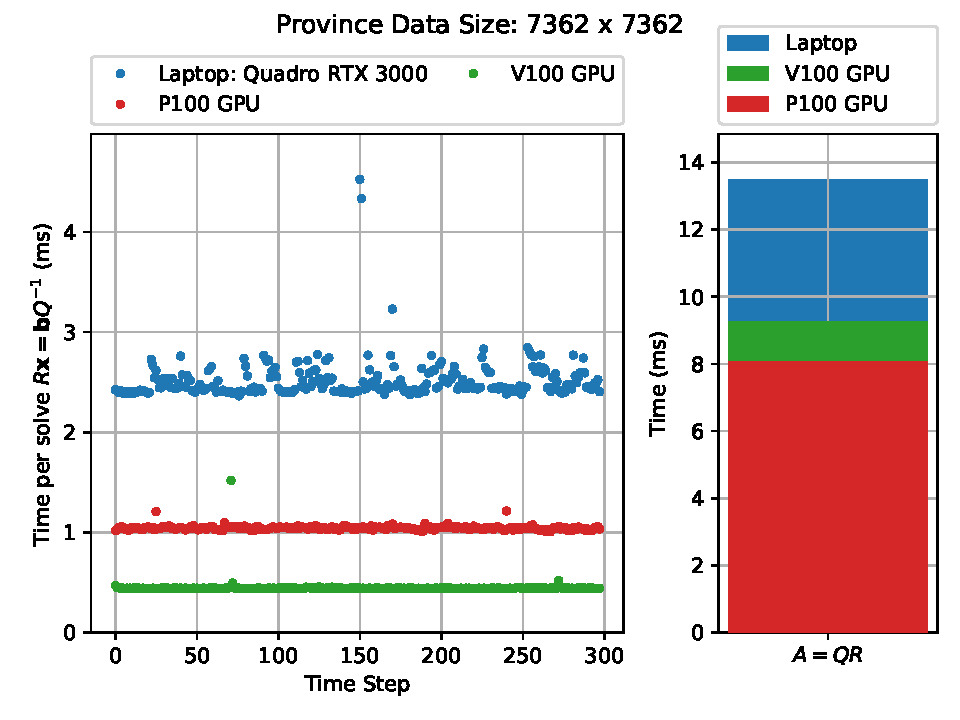
\includegraphics[width=\textwidth]{C:/Users/bradc/Documents/MHI/Output/FullTimings.pdf}
    \end{subfigure}
    \;
    \begin{subfigure}{0.48\textwidth}
        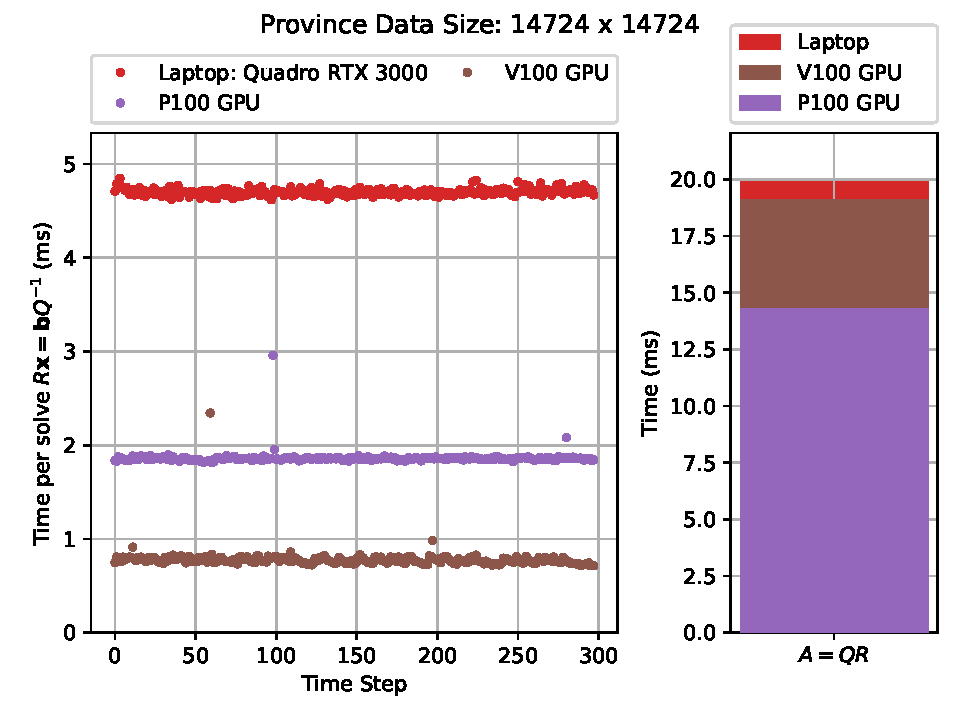
\includegraphics[width=\textwidth]{C:/Users/bradc/Documents/MHI/Output/FullTimings_n2.pdf}
    \end{subfigure}
    \\
    \begin{subfigure}{0.48\textwidth}
        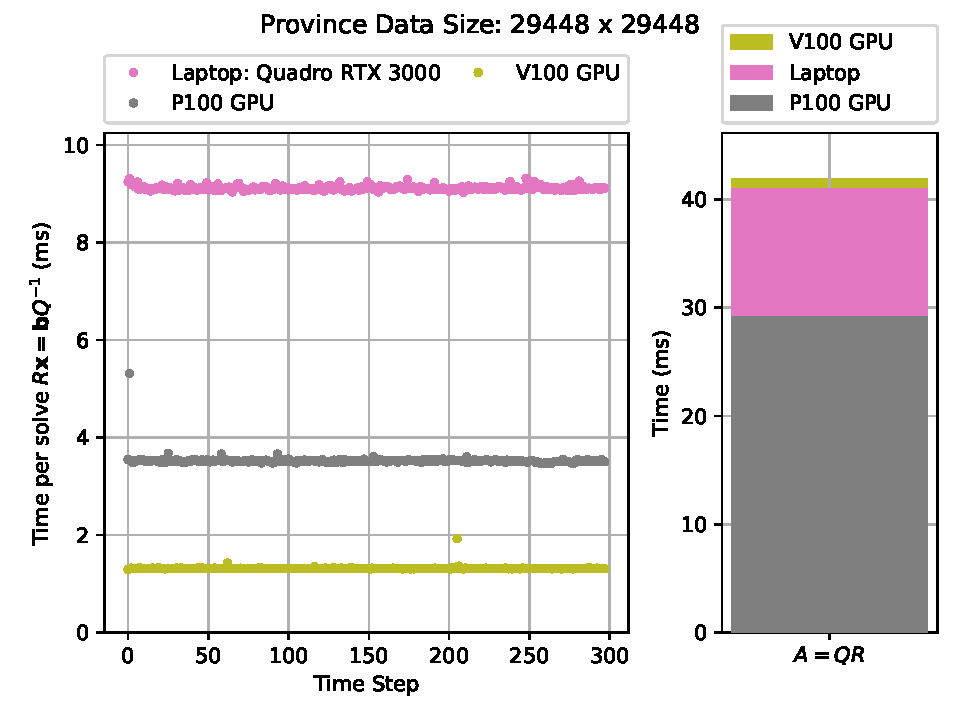
\includegraphics[width=\textwidth]{C:/Users/bradc/Documents/MHI/Output/FullTimings_n4.pdf}
    \end{subfigure}
    \;
    \begin{subfigure}{0.49\textwidth}
        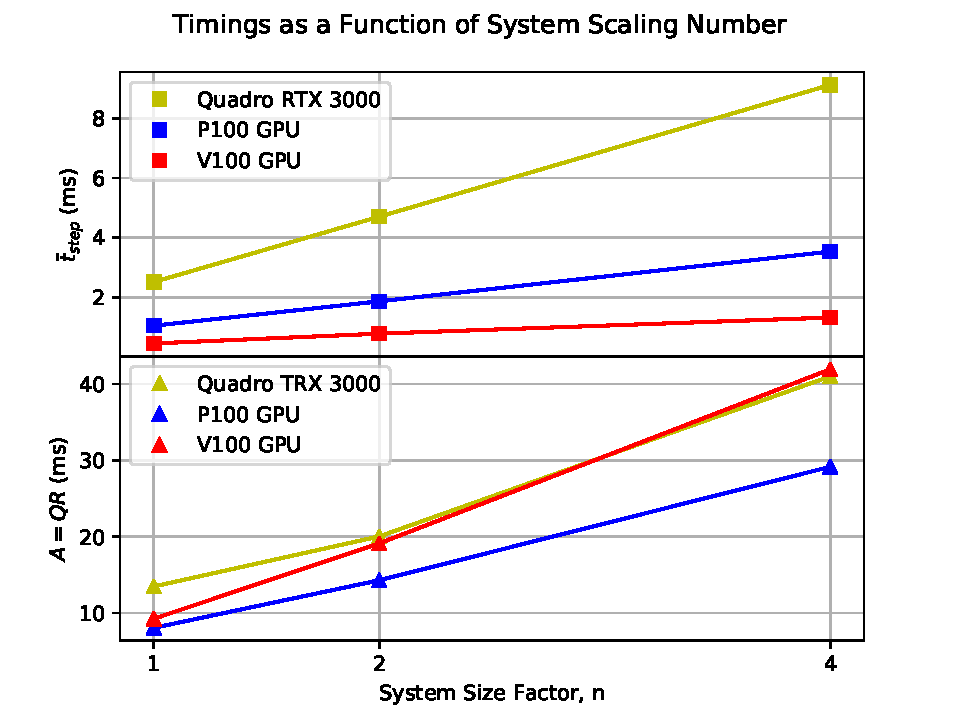
\includegraphics[width=\textwidth]{C:/Users/bradc/Documents/MHI/Output/TimingScales.pdf}
    \end{subfigure}
    \caption{{\it Top and bottom left}: per-time step solving time and matrix factoring time for each of the 
    three GPUs tested. The system size is given at the top of each plot. The original size of the 
    \emph{Province} data set is 7362~x~7362, and subsequent systems are either twice or quadruple 
    this size. {\it Bottom right}: the average per-time step solving time and matrix factoring time for
    each of the GPUs tested as a function of system size facor. A value of $n=1$ corresponds to the 
    original \emph{Province} system size.}
    \label{f:all_timings}
\end{figure}
        
\end{document}
